\newpage
\section{Revisão da Teoria}

Para o conversor Buck em modo contínuo, o valor a ser ajustado de modo a compensar a tensão de saída é a largura do pulso de chaveamento do conversor, chamado de razão cíclica ($D$). Sendo $D$ a razão entre o tempo de condução do transistor e o período de chaveamento:
\[
    D = \frac{T_{on}}{T}.
\]

O ajuste de $D$ é feito por um bloco de controle, o qual usa uma tensão de erro ($V_{erro}$) para calcular o valor de $D$ que fará com que a tensão de saída se aproxime da desejada, reduzindo assim as variações na tensão de saída.

\subsection{Tensão de erro}

\begin{figure}[H]
    \centering
    \caption{Circuito para gerar a tensão de erro.}
    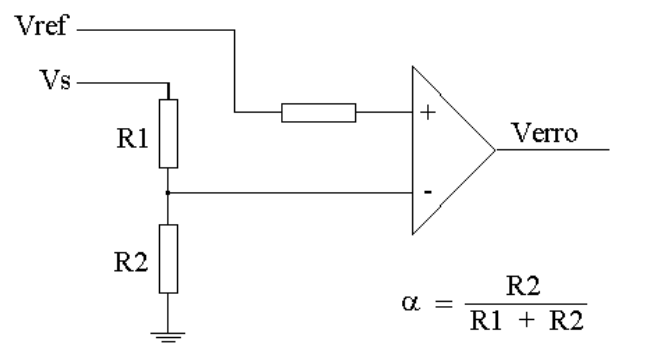
\includegraphics[scale=0.4]{verro}
    \label{fig:verro}
\end{figure}

A tensão de erro é obtida comparando-se uma tensão de referência (a qual é conhecida) a uma tensão de ajuste. Para o controlador em malha aberta, $V_s$ na figura \ref{fig:verro} é gerada com o auxilio de um potenciômetro. Em circuitos mais elaborados (controlador em malha fechada), $V_s$ é provindo a partir da tensão de saída do conversor.

No circuito da figura \ref{fig:verro}, o amplificador operacional atua comparando a tensão de entrada $V_s$, multiplicada pelo ganho $\alpha$, a tensão de referência $V_{ref}$. O valor de $V_{erro}$ é utilizado para ajustar o valor de $D$ de modo que:
\[
    V_{ref} - V_s \alpha = 0.
\]

\subsection{Circuito de controle}

O CI empregado nesse trabalho (SG3524) possui uma topologia semelhante a apresentada na figura \ref{fig:ctl}. Seu funcionamento explicado abaixo.

\begin{figure}[H]
    \centering
    \caption{Topologia do circuito de controle.}
    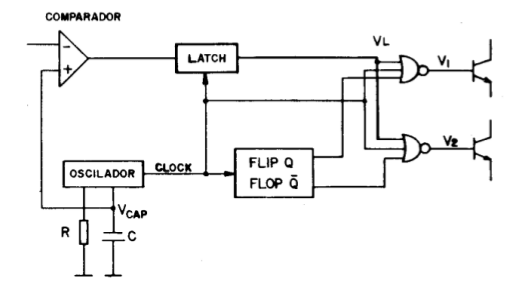
\includegraphics[scale=0.6]{ctl}
    \label{fig:ctl}
\end{figure}

O oscilador (cuja frequência de oscilação é determinada por $R$ e $C$) fornece um pulso positivo de curta duração (durante a descarga do capacitor C) o qual ocasiona o \textit{resset} do \textit{latch}, muda a condição de saída do \textit{flip-flop} e inibe as saídas. O estado do comparador é utilizado para armazenar o estado do comparador. Quando o \textit{latch} recebe um pulso do oscilador, o mesmo vai para o estado zero e se mantém assim até que a tensão de erro seja menor do que $V_c$. Quando a tensão de erro se torna menor que $V_c$, o \textit{latch} passa para um nível alto até o próximo pulso de \textit{clock}.
O \textit{flip-flop}, por sua vez, garante que somente uma das duas saídas disponíveis estará ativa, possibilitando o uso do circuito em conversores do tipo \textit{push-pull}. Vale notar que, ao se utilizar somente uma saída, temos uma variação máxima da largura de pulso de 50\%, porém, se utilizarmos as duas saídas em paralelo, temos 100\% de variação.

A figura \ref{fig:3524} mostra o esquema interno do CI SG3524, onde é possível observar a semelhança com a topologia analisada.

\begin{figure}[H]
    \centering
    \caption{Circuito integrado SG3524.}
    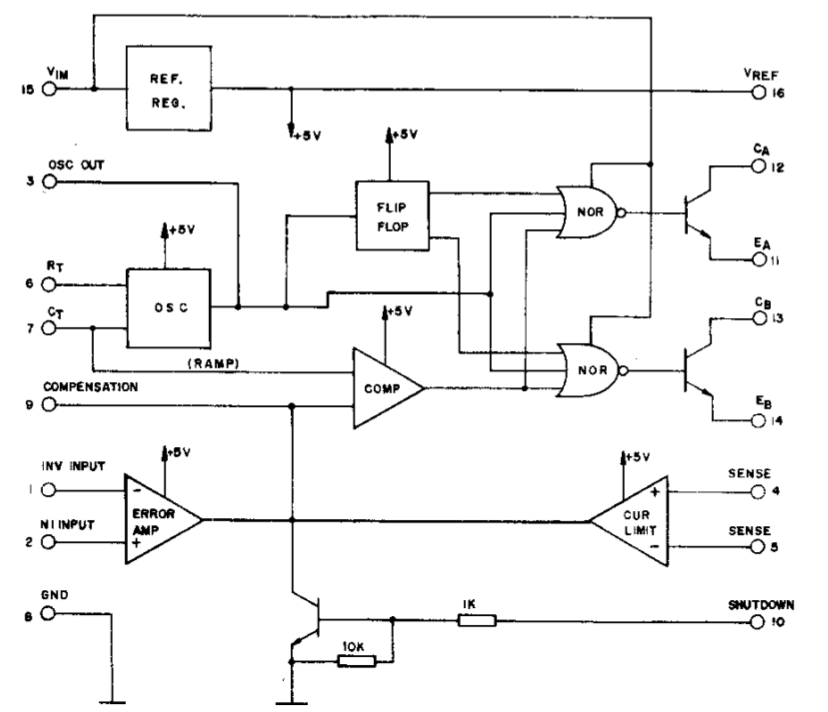
\includegraphics[scale=0.4]{3524}
    \label{fig:3524}
\end{figure}
